\section{Experimental Results}

\begin{figure*}[t]
	\centering
	\vspace{-3pt}
	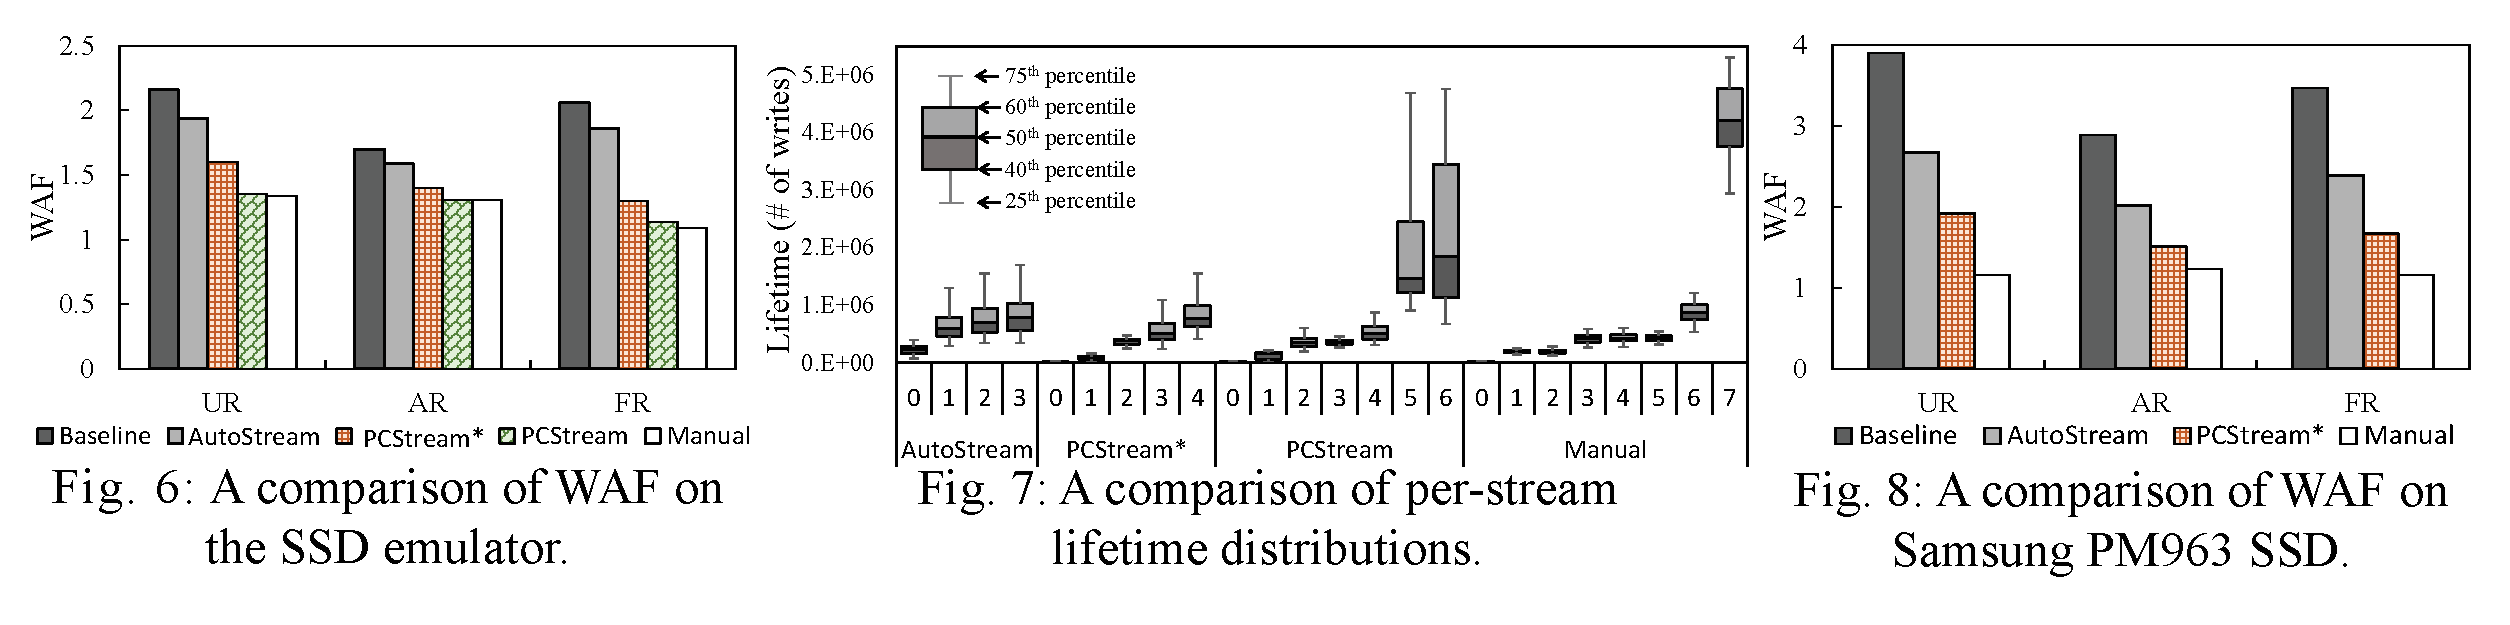
\includegraphics[width=1\textwidth]{figure/expfig}
%	\subfloat[\scriptsize{A comparison of WAF on the SSD emulator}.]{\label{fig:result_emul}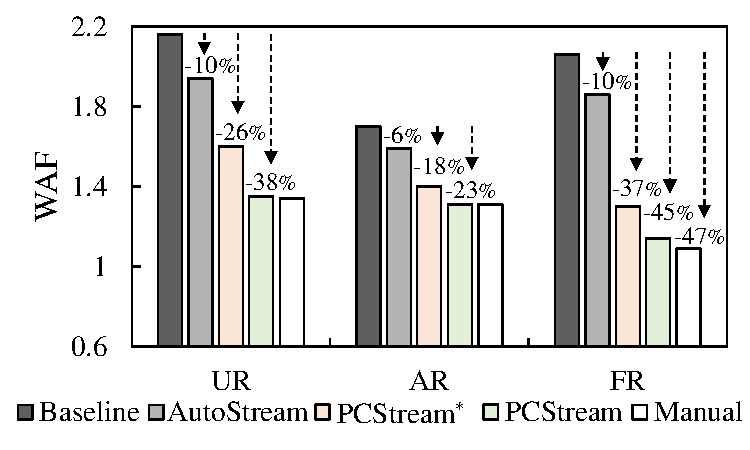
\includegraphics[width=0.33\textwidth]{figure/result_emul}}
%	\subfloat[\scriptsize{A comparison of WAF on PM963}.]{\label{fig:result_ssd}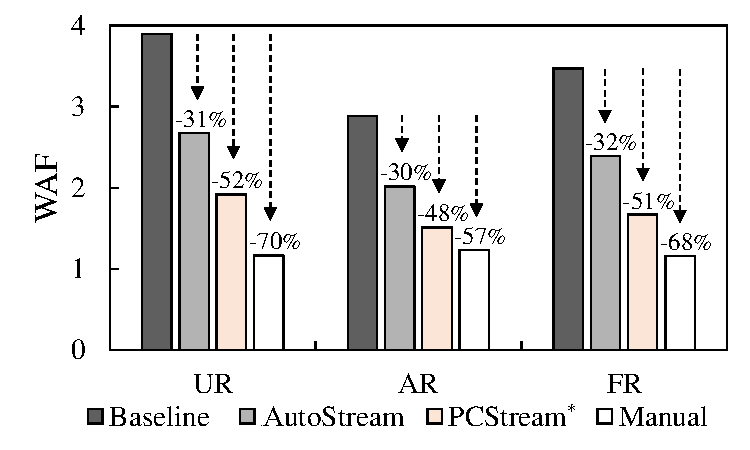
\includegraphics[width=0.33\textwidth]{figure/result_ssd}}
%	\subfloat[\scriptsize{A lifetime comparison of each stream}.]{\label{fig:streamlifetime}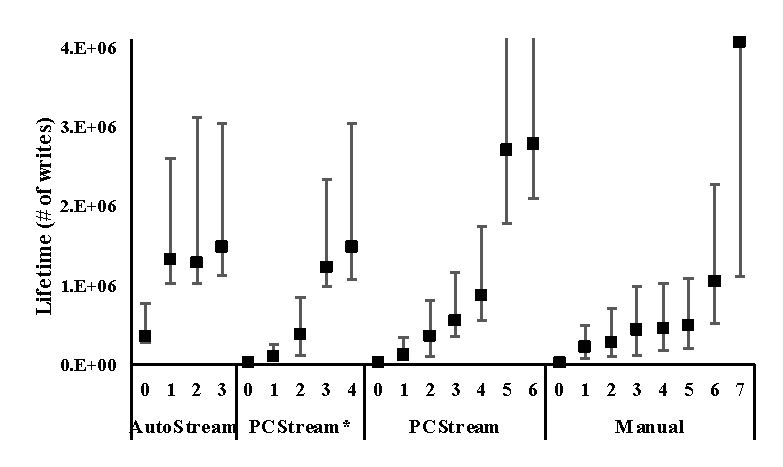
\includegraphics[width=0.33\textwidth]{figure/streamlifetime}}
%	\vspace{-10pt}
%	\caption{The WAF comparison on the emulator.}
	\label{fig:exp}
	%\vspace{-36pt}
\end{figure*}

For our experiments, we have implemented \textsf{\small PCStream} in the Linux kernel
4.5.  For an objective evaluation, we compared \textsf{\small PCStream} with three
existing schemes: \textsf{\small Baseline}, \textsf{\small Manual}~\cite{MultiStream}, and
\textsf{\small AutoStream}~\cite{AutoStream}.  \textsf{\small Baseline} stands for a legacy
SSD that does not support a multi-stream feature. \textsf{\small Manual} is a RocksDB
implementation which is manually optimized for multi-streamed SSDs.
\textsf{\small AutoStream} is an LBA-based data separation technique which is
implemented at the device driver layer. To understand the impact of the
two-phase assignment, in addition, we compared \textsf{\small PCStream} with
\textsf{\small PCStream$^{*}$} which excluded the two-phase assignment feature.

For benchmarks, we have used three scenarios of \texttt{db\_bench} of RocksDB:
Update-Random (\texttt{UR}), Append-Random (\texttt{AR}), and Fill-Random
(\texttt{FR}) scenarios.  For key-value pairs already stored in the SSD,
\texttt{UR} updates values for random keys, creating many
read-modify-writes in the SSD.  \texttt{AR} is similar to \texttt{UR}, except
that it performs the update of values for growing keys. \texttt{FR} writes
key-value pairs to the SSD in a random key order.

\subsection{Experimental Setting}

\subsection{WAF Comparison}

We carried out a set of experiments using an SSD emulator which is based on the
open flash development platform~\cite{AMF}.  
The SSD emulator emulates the behaviors of an SSD using host DRAM in the kernel level. Thus, it not only allows us to easily add new features, but enables to analyze detailed internal activities of an SSD. 
For our evaluations, we extended the SSD emulator to support a multi-streamed feature.
We assume that the SSD emulator supports up to 8 streams (as with Samsung PM963 which was used in our experiments). %shane part
We enhanced the original emulator so that it supported a multi-streamed feature as well as the two-phase stream assignment.  The number of streams supported by the emulator was 8.  
The SSD emulator provided 12 GB capacity with 4 channels and 4 ways, and there were 8192 flash blocks, each of which was composed of 384 4-KB pages.  


We compared WAF of the existing techniques with \textsf{\small PCStream} for the three
scenarios, and the result is shown in Fig. 6.  
\textsf{\small PCStream} was quite effective in reducing WAF, 
thus achieving an equivalent level of the WAF reduction as in \textsf{\small Manual}.  
For example, both \textsf{\small PCStream} and \textsf{\small Manual} reduced WAF by 38\% over \textsf{\small Baseline} for the \texttt{UR} case. 
Compared with \textsf{\small AutoStream}, \textsf{\small PCStream} was more effective, reducing WAF more by 35\% on average.  
\textsf{\small PCStream} outperformed \textsf{\small AutoStream} by reducing WAF by 35\% on average.
Fig. 6 also indicates that the two-phase stream assignment technique is effective.  
\textsf{\small PCStream} outperformed \textsf{\small PCStream$^{*}$} by 12\% on average in the WAF reduction.
As shown in Fig. 6, \textsf{\small PCStream$^*$} reduced WAF by up to 30\% over \textsf{\small AutoStream}.  
The result shows that separating short-lived data (e.g., log and flush) from long-lived one (e.g., compaction) using PC was quite effective in reducing WAF.  Moreover, \textsf{\small PCStream} even showed similar WAF to \textsf{\small Manual}, reducing it by up to 38\% over \textsf{\small AutoStream}.  
This additional gain of \textsf{\small PCStream} over \textsf{\small PCStream$^{*}$} came from isolating long- and short-lived data in separate blocks 
by moving the long-lived data of the compaction-activity PC to substreams during GC at the SSD.

\subsection{Per-stream Lifetime Distribution}

In order to better understand how \textsf{\small PCStream} achieved a high reduction in WAF, 
we measured per-stream lifetime distributions under each technique for the \texttt{UR} scenario.
Fig. 7 shows a box plot of data lifetimes from the 25th percentile to the 75th percentile.
As shown in Fig. 7, 
streams in \textsf{\small PCStream} are divided into two groups, 
$G1$ = $\{$0, 1, 2, 3, 4$\}$ and $G2$ = $\{$5, 6$\}$, 
where $G1$ includes streams with short lifetimes and small variances (i.e., streams 0, 1, 2, 3, and 4) 
and $G2$ includes streams with large lifetimes and large variances (i.e., streams 5 and 6).  
Since the GC copy cost is affected by how data in $G1$ and $G2$ are mixed into the same block, 
\textsf{\small PCStream} can significantly reduce the GC overhead 
by avoiding such data mixtures in the same block by separating $G1$ and $G2$ into different streams. 
On the other hand, in \textsf{\small AutoStream}, 
three streams (i.e., streams 1, 2, and 3) show similar lifetime distributions with large variances 
without a distinct data separation pattern.
In Fig. 7, we can also observe the effect of substreams.  
Streams 3 and 4 of \textsf{\small PCStream$^{*}$}, 
which have large variances in lifetimes, are split into two substreams 5 and 6 in \textsf{\small PCStream}.
This split reduces variances of streams 3 and 4, thus reducing the GC copy cost.  

\subsection{Effect of IOS Management}

\subsection{TBD - additional experiment}
